\section{What is Bureaucracy?\label{sec:define-bureaucracy}}

While you may know it when you see or experience bureaucracy,\footnote{See the Wikipedia entry for \href{https://en.wikipedia.org/wiki/I_know_it_when_I_see_it}{``I know it when I see it."}} 
\index{Wikipedia!I know it when I see it@\href{https://en.wikipedia.org/wiki/I_know_it_when_I_see_it}{I know it when I see it}}
for this book definitions are helpful. Throughout the book I'll refer back to these definitions as I explain concepts needed to understand bureaucracy.

\index{bureaucracy!definition of}
\iftoggle{glossaryinmargin}{\marginpar{[Glossary]}}{}
\iftoggle{glossarysubstitutionworks}{\Gls{bureaucracy}}{Bureaucracy}
involves the creation and execution of 
\iftoggle{glossarysubstitutionworks}{\glspl{policy}}{policies} for managing shared resources. 
Creating and carrying out policies usually involves multiple people, each having a specialized role. Motivated by scalability (how many widgets), complexity (number of tasks per widget), or latency (time per widget), members with distinct roles form a hierarchical organization to facilitate coordination. The organization has control over the disbursement of resources relevant to the society the organization works within, or the organization administers a policy within that society. Resources managed by the organization are either tangible (e.g., water, air, land) or intangible (expertise, e.g., food inspection, teaching mathematics, painting cars; information, e.g., census results).  

Bureaucracy relies on a combination of \href{https://en.wikipedia.org/wiki/Quid_pro_quo}{quid pro quo}
\index{Wikipedia!quid pro quo@\href{https://en.wikipedia.org/wiki/Quid_pro_quo}{quid pro quo}}
(carrot) and coercion of subjects (stick). The coercion can be a threat of physical violence or threat of sanction -- namely removal from the process. This interpretation applies even within bureaucratic organizations to the member bureaucrats, where threat of sanction can be formal (up to removal) or informal (outcast from the group of professional bureaucrats).

Bureaucracy is not limited to government. Non-profit organizations, volunteer groups, commercial companies, and even small teams of people can invoke bureaucratic tendencies. The existence of bureaucracy is independent of an organization's purpose and independent of whether money is involved. Carrying out someone else's subjectively defined policy will require you to make subjective decisions regarding execution and enforcement. 

\subsection*{Roles in Bureaucracy}

Distinct roles can be identified within the description of bureaucracy.
\index{bureaucracy!roles}
\iftoggle{glossarysubstitutionworks}{\Gls{core bureaucracy}}{Bureaucracy} involves 
a \gls{policymaker}, 
a policy enforcer (the bureaucrat), and the person upon whom policy is inflicted 
(the \gls{subject}). 
The policy is typically for a shared or contended resource. In the context of government, the policy creator can be either a politician or a bureaucrat. In the context of a family, the primary caretaker usually sets policies. The assignment of roles to individual people is not fixed -- the assignment depends on the scenario. 

\begin{figure}
    \centering
    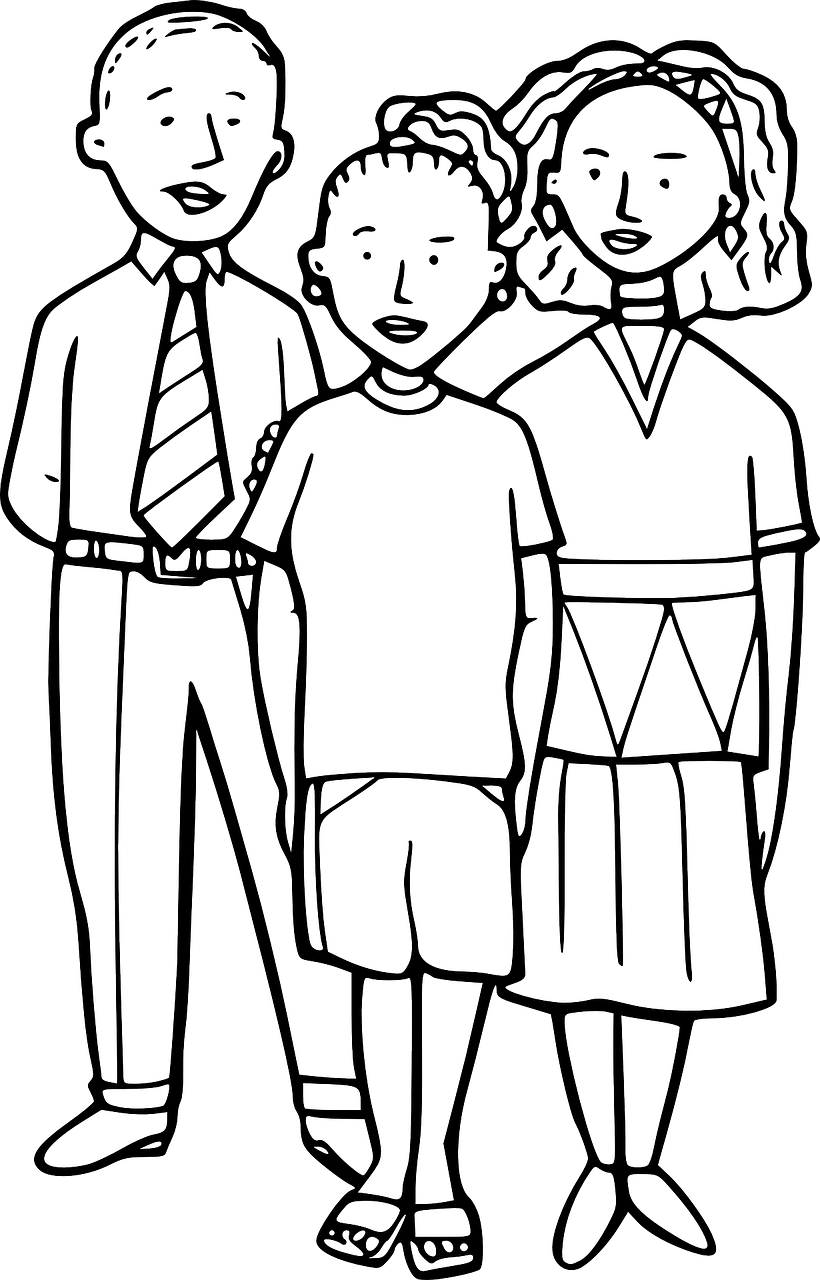
\includegraphics[width=.6\textwidth]{images/family-father-mother-daughter-28725_1280_pixabay.png}
    \caption{This family consists of a policymaker, a bureaucrat who enforces policies, and the subject of bureaucracy. Which person has which title depends on the situation. For example, if Mom says no dessert until after the daughter eats her peas, then Dad helps enforce that policy. The shared resource being managed is the dessert. }
    \label{fig:family-of-bureaucrats}
\end{figure}

A crucial aspect of bureaucracy is the separation of roles: policymaker, bureaucrat, and subject have to be separate people. This separation creates 
\href{https://en.wikipedia.org/wiki/Conflict_of_interest}{conflicts of interest}  
\index{Wikipedia!conflict of interest@\href{https://en.wikipedia.org/wiki/Conflict_of_interest}{conflict of interest}}
that wouldn't otherwise occur. For example, suppose you need to design a security policy for a computer, and you then want the policy reviewed. If those two roles are filled by the same person there's no conflict of interest. 
One person creating a policy and a different person enacting policy is necessary for bureaucracy to arise. Similarly, the person enacting policy must be separate from the person upon whom the policy is inflicted; otherwise who could complain?

While three people is the minimum for bureaucracy, bureaucrats often congregate. 
An organization comprised of bureaucrats typically has a leader -- something like a Chief Executive Officer (CEO). Because the CEO doesn't know everything and can't make all the decisions a variety of management styles exist to spread the responsibility within the organization and leverage the diffuse expertise. Which management style is most effective depends on the personalities of people involved. Regardless of management style the challenges of distributed knowledge and distributed 
\href{https://en.wikipedia.org/wiki/Decision-making}{decision-making} 
\index{Wikipedia!decision-making@\href{https://en.wikipedia.org/wiki/Decision-making}{decision-making}}
are present. 

The roles of policymaker, bureaucrat, and subject apply within organizations comprised of bureaucrats. That mapping of labels can initially be confusing but aligns with the personal experience of bureaucrats. As an example, a supervisor at a state agency is a bureaucrat, but he sets policy for you and your team members regarding interactions with other teams in the state agency. In this scenario bureaucrats on other teams are the subjects of the policy you're enforcing.

%An  is called bureaucratic.
The main character within a bureaucratic organization is the \gls{bureaucrat} -- the person who is a member of an organization and is responsible for subjectively enacting policy on someone else's behalf. The person that a bureaucrat's decisions are inflicted on is a \gls{subject}.  Depending on context, a subject may be a student (when the bureaucrat is a teacher)
\index{exemplar!school}
or a subject may be a citizen if the bureaucrat is a police officer 
\index{exemplar!law enforcement officers (LEO)}
or government official. Sometimes a bureaucrat's decisions are inflicted on other bureaucrats-as-subjects, such as when a Chief of Police creates guidelines for police in their district, or when a senior diplomat sets policies for embassy employees. 

While the roles of policy maker, bureaucrat, and subject are pervasive in a variety of contexts, bureaucrats usually avoid using the pejorative label. Typically formal titles are used that are associated with a specialization. Titles are more than just labels; titles impersonalize interactions, displacing the need for interpersonal relationships. This impersonalization is what enables the value of bureaucracy, while also causing a negative perception. As a subject engaging with a bureaucratic organization your relationships are irrelevant -- you get access to the shared resource regardless. The rest of this book uses the label of bureaucrat in a neutral sense even though socially there is a negative connotation.  

A \gls{bureaucrat} \iftoggle{glossaryinmargin}{\marginpar{[Glossary]}}{}%
subjectively interprets policies made by someone else and has discretionary enforcement.  
Let's break that previous sentence down piece-by-piece. First, ``subjective interpretation'' means a person is deciding how to do something. Subjectivity arises from different reasons one person might choose an option over a competing alternative.  A \gls{policy} \iftoggle{glossaryinmargin}{\marginpar{[Glossary]}}{}%
is a set of actions regarding a shared resource in a given circumstance. 
%An \gls{organization} is the collection of people for who the policy is made. 
Discretionary enforcement means the bureaucrat chooses how to apply the policy in specific circumstances. 

Often more than one bureaucrat is inflicting a policy, in which case there's a need to facilitate coordination of stakeholders by applying specialized knowledge. 
Facilitating coordination means getting multiple people in different roles
%(or sometimes a person at different instances in time) 
to accept a decision about the shared resource. The stakeholders are people who care about the application of the action in each circumstance.  


The summary above is still pretty dense, so the rest of the book is spent expanding the nuances and implications of this definition.

\subsection*{Consequences of the Definition of Bureaucracy}

\textit{Armed with the definitions and roles, let's explore the consequences of this paradigm.}

Bureaucracy is neither good nor bad. Bureaucracy is not tied to politics, nor is bureaucracy specific to an institution (e.g., corporations, governments, academia). The definition of bureaucracy used in this book is independent of government. Bureaucracy is not defined to be efficient, nor does it have to be inefficient. Bureaucracy is not restricted to paperwork, record keeping, quantification, or gathering metrics. Nothing in this definition involves paperwork or an office building. Definitions that limit the concept of bureaucracy to specific contexts result in a decreased ability to describe complex, large-scale organizations of humans. If your definition of bureaucracy is limited to government, then you'll be confused by similar behavior showing up in small groups of volunteers and in commercial businesses.

Bureaucracy is about delegation of control, communication, decision-making, coordination, and processes. 
A vital aspect of bureaucracy is that everything is arbitrary -- as determined by humans.



\begin{figure}
    \centering
    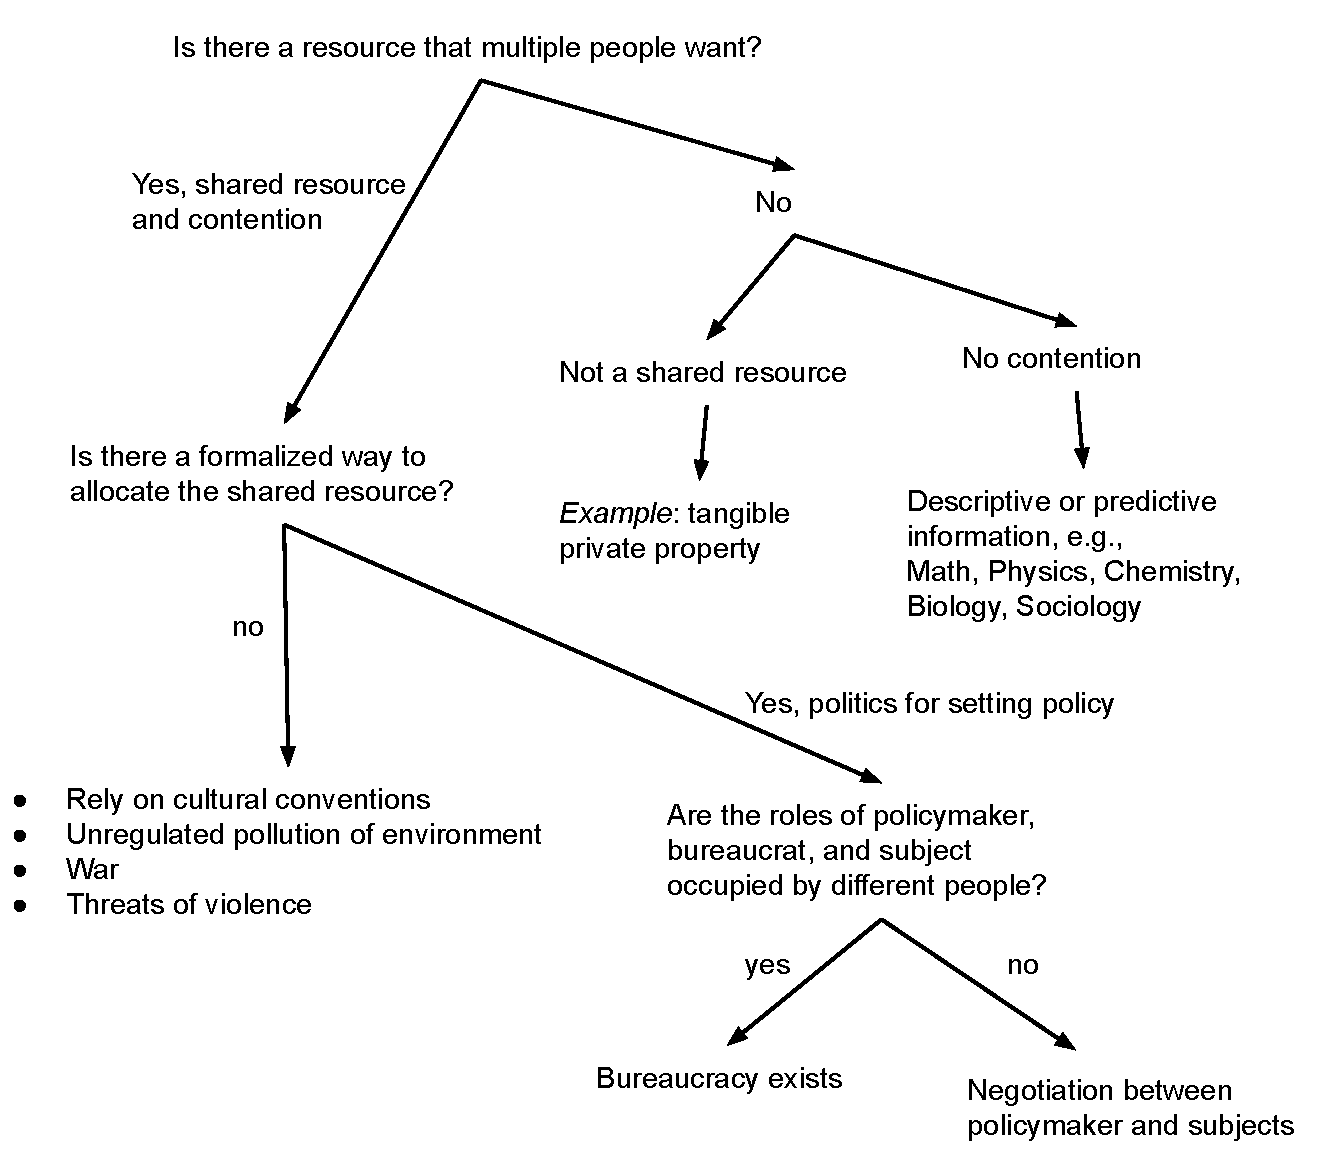
\includegraphics[width=1.05\textwidth]{images/relation_between_shared_resource_and_bureaucarcy.pdf}
    % DEPRECATED: am_I_a_bureaucrat.pdf
    \caption{This book focuses on bureaucracy but there are ways to manage access to shared resources that are not bureaucratic.  
    This decision tree shows ways that are and are not bureaucratic. Start from the top, then evaluate the sequence of questions to determine which label applies to your situation.
    One endpoint on the left bottom is 
    the 
    \href{https://en.wikipedia.org/wiki/Tragedy_of_the_commons}{tragedy of the commons}  
    \index{Wikipedia!tragedy of the commons@\string\href{https://en.wikipedia.org/wiki/Tragedy_of_the_commons}{tragedy of the commons}}
    -- the case of a shared resource with no constraints on use. Then someone will try to get away with behavior that is harmful to the community of users. }
    \label{fig:am-I-a-bureaucrat}
\end{figure}

The consequence of subjectivity is that everything is negotiable. Bureaucracy relies on negotiation to adjust to nuanced circumstances not foreseen when policies were designed.  You (whether in the role of a subject or a bureaucrat) need to know who to negotiate with and how to negotiate the changes you seek. 

Bureaucracy is arbitrary, but there are actual rules that constrain us. The mathematical physics that describe nature are not negotiable. Everything in your environment is either naturally occurring macroscopic emergent phenomena (e.g., chemistry, biology) or humans making up labels and norms. Distinguishing the two is critical to knowing what you can change and what you have to work within. See Figure~\ref{fig:am-I-a-bureaucrat}\iftoggle{haspagenumbers}{ on page~\pageref{fig:am-I-a-bureaucrat}}{} for an illustration of the decision sequence.

Bureaucracy arises when there is no standard, objectively quantifiable feedback mechanism for individual participants in the organization. This aspect is why governments, schools, and prisons are characterized as bureaucratic. 
\index{exemplar!school}
\index{exemplar!prison}
The military doesn't rank soldiers by ``number of enemies killed'' and is bureaucratic. 
\index{exemplar!military}
Even profit-driven commercial organizations are bureaucratic when the actions of individual employees are not coupled to the metrics of profit. %Government bureaucracy gets a negative reputation because of the interaction with public, whereas corporate shenanigans are considered domain specific rather than systemic.

%In fact, some issues are systemic to organizations of people that rely on distributed knowledge and distributed decision-making.

Profit-based feedback makes some roles in a business context slightly more predictable and sensible. Even in that situation there are subjective trade-offs like what costs get externalized and whether to focus on long-term profit versus short-term profit. 

The concept of bureaucracy is most visible for complex recurring situations involving many people and the control of a shared resource. The friction of bureaucratic processes can be lower when there are only a few people involved (``I'm just talking to my collaborator," or ``I'm just buying groceries from a clerk at the store,'' or ``I'm using a website for a government service''), but there is a gradient to more obvious instances of bureaucracy. Bureaucratic tendencies are observable at small scale, but in that limit it becomes difficult to distinguish what is attributable to the participants involved.

Operating within an organization of bureaucrats feels different from other parts of your life because of the interdependence and loss of autonomy. 
Modern conveniences are designed to hide bureaucracy and create the illusion of independence.
Aspects of modern life like electricity, water, sewage, safety, and entertainment all operate at a scale that makes dependence on other humans almost invisible. You probably don't know the person who wired your house, runs the electrical power plant, monitors the flow of clean water, or treats sewage. A breakdown of those services is a 
\href{https://en.wikipedia.org/wiki/Leaky_abstraction}{leaky abstraction}.
\index{Wikipedia!leaky abstraction@\href{https://en.wikipedia.org/wiki/Leaky_abstraction}{leaky abstraction}}
\iftoggle{WPinmargin}{\marginpar{$>$Wikipedia: Leaky abstraction}}{}

\ \\

Bureaucracy arises when management of a shared resource is necessary.
That resource can be external to the organization or internal to the organization. Examples of external shared resources include mail delivery for the \href{https://en.wikipedia.org/wiki/United_States_Postal_Service}{USPS},%
\index{exemplar!United States Postal Service (USPS)}%
\iftoggle{WPinmargin}{\marginpar{$>$Wikipedia: USPS}}{}
\index{Wikipedia!United States Postal Service@\href{https://en.wikipedia.org/wiki/United_States_Postal_Service}{United States Postal Service}}
public safety for the \href{https://en.wikipedia.org/wiki/Federal_Bureau_of_Investigation}{FBI}, 
\index{exemplar!Federal Bureau of Investigation (FBI)}%
\index{Wikipedia!Federal Bureau of Investigation@\href{https://en.wikipedia.org/wiki/Federal_Bureau_of_Investigation}{Federal Bureau of Investigation}}%
and the environment for the \href{https://en.wikipedia.org/wiki/United_States_Environmental_Protection_Agency}{EPA}. 
\index{exemplar!Environmental Protection Agency (EPA)}
\index{Wikipedia!Environmental Protection Agency@\href{https://en.wikipedia.org/wiki/United_States_Environmental_Protection_Agency}{Environmental Protection Agency}}%
The focus of this book is on resources internal to an organization. Intangible resources internal to a bureaucratic organization include attention, skill, and expertise. Those shared internal resources get quantified as time, money, and staffing. While talking about time and money and staffing are easy to make trade-offs with, keep in mind they are proxy measures for the central intangible resources like attention and expertise.

\subsection*{Bureaucracy is Necessarily Complicated}

Bureaucracy is a system for distributed knowledge\footnote{``[Bureaucracy] is designed to take in and digest different pieces of information in far greater quantity than the human head alone can hold and produce from this mass of differentiated data, a useful synthesis."~\cite{1966_Morison}} 
and distributed decision-making. 
\index{bureaucracy!definition of}
That is in contrast to easier-to-understand concepts like centralized knowledge and centralized decision-making. A government run by dictatorship is easier to conceptualize than democracy because there is a central character around which a narrative can be formed. Similarly, stories about the \href{https://en.wikipedia.org/wiki/Chief_executive_officer}{CEO} 
\index{Wikipedia!Chief Executive Officer@\href{https://en.wikipedia.org/wiki/Chief_executive_officer}{Chief Executive Officer}}%
\iftoggle{WPinmargin}{\marginpar{$>$Wikipedia: Chief executive officer}}{}
of a company are easier than capturing the thousands of interactions conducted by the many employees of that company. The vast majority of the work an organization does is coordinated and carried out by people other than the CEO. Most of what is known within an organization is known by people other than the CEO. Linear storytelling with a small number of main characters does not map well to the complexities of bureaucracy. 

\ \\

If you think bureaucracy sucks and it should be removed or replaced,  consider the parable of 
\href{https://en.wikipedia.org/wiki/G._K._Chesterton\%23Chesterton\%27s_fence}{Chesterton's fence}~\cite{1929_Chesterton}. 
\label{concept:chestertons_fence}
\index{Wikipedia!Chesterton's fence@\href{https://en.wikipedia.org/wiki/G._K._Chesterton\%23Chesterton\%27s_fence}{Chesterton's fence}}
\iftoggle{WPinmargin}{\marginpar{$>$Wikipedia: Chesterton's fence}}{}
\begin{quote}
``There exists ... a fence or gate erected across a road. The more modern type of reformer goes gaily up to it and says, `I don't see the use of this; let us clear it away.' To which the more intelligent type of reformer will do well to answer: `If you don't see the use of it, I certainly won't let you clear it away. Go away and think. Then, when you can come back and tell me that you do see the use of it, I may allow you to destroy it.'"
\end{quote}
You need to understand the historical evolution of each process that your organization relies on to understand why bureaucracy exists.
